\chapter{Introduction}
\label{chap:introduction}
% \subtitle{Building a distributed reputation system as the basic infrastructure for creating trust 
% between relative strangers for the future digital economy.}

% \paragraph{Abstract.} Trust enables cooperation which in the long-term increases welfare for all 
% parties, but centralization creates an unhealthy information and, thus, power asymmetry. The future 
% digital economy will be driven by global cooperation between relative strangers; that cooperation 
% will be facilitated by distributed reputation systems without central ownership or control. This 
% work extends the scalable TrustChain fabric with an explicit, unambiguous, public representation of 
% the entities' states, thereby making sharing of information incentive-compatbile and putting another
% pillar for the trustful internet in place.

% 1. Since the ground-breaking work of Darwin we know that evolution of species is guided by natural selection, so mutation and inheritance lead to the strongest variation surviving. However, the classic view of the strongest survives does not explain how cooperation can occur, which requires some sort of altruism. Game theory explains …
%  Nowak, Axelrod, 

The theory of evolution has been studied for many centuries as it is a bewildering thought that from
the raw elements that make up our planet a living organism arose and evolved into our sophisticated,
complex society. Since the ground-breaking work of Darwin some mechanisms that fuelled that
evolution have been widely accepted in the scientific community, namely natural selection, the 
survival of the strongest random mutation of a species that inherits its phenotype to the next 
generation, creating a fitter generation. This theory about competition between individuals was the
accepted truth about evolution but in the late 1960s doubts arose about the completeness of this 
theory. When looking at group behavior in species one will find that cooperation is a common theme
among related individuals, yet there is no place for cooperation in the classic Darwin 
theory.\cite{Axelrod1390} In their work Axelrod and Hamilton \cite{Axelrod1390} 
analyze how to combine the seemingly inferior individual's strategy of cooperating with the goal to 
maximize fitness. At the basis of their experiments is a game called Prisoner's 
Dilemma~\cite{chammah1965prisoner}, in which two players can choose to cooperate or defect: if both
cooperate they fare best, if both defect they fare okay, yet if one cooperates and the other defects
the cooperator farest the worst. This creates a social dilemma: not knowing what the other does,
makes defecting the only reasonable strategy, yet if both would trust each other to cooperate, they
would both win. Axelrod and Hamilton ran experiments on this game with multiple rounds with
different strategies and found that if the game is played multiple rounds with the possibility of 
meeting the same partner again in the future, cooperation between players can be established and be
superior. Later research showed that this direct form of reciprocity, the act of returning a deed,
is only one form of cooperation found in species and human behavior. Nowak and 
Martin~\cite{nowak2006five} defined five forms in which cooperation can occur: kin selection, direct
reciprocity, indirect reciprocity, network reciprocity and group reciprocity. Conceptually these 
forms can be described like this:

\begin{itemize}
    \item kin selection: we help those that share our genes
    \item direct reciprocity: I help you, you help me
    \item indirect reciprocity: I help you, somebody helps me
    \item network reciprocity: neighbors help each other
    \item group selection: A group, in which members help each other, survives
\end{itemize}

These mechanisms for fostering cooperation entail an important concept: trust. We trust those that
are close to us and we trust those that we have had succesful interactions with before. If two
entities trust each other, they are able to cooperate and as a result, prosper. If trust is broken
both parties will fare worse. 

% 2. Trust in economy and digital markets …. Advance of sharing economy, ….. When talking about trust, indirect reciprocity is the method of creating cooperation. Mui created a first mathematical model which relates reputation, trust and reciprocity. According to that model reputation stems from the history of encounters 
% Mui, Martin

Trust and cooperation lay the basis for human societies and have a long history. A prominent example
is the evolution of economy as shown in Figure \ref{fig:economy}. In the pre-industrial age, most economy and trade was done in local
communities with families that trusted each other over generations and traders that returned year
after year. During industrial and post-industrial age companies have largely replaced local 
producers and are trusted by millions of customers based on their brand name. Nowadays, in the 
information age, internet companies allow people to connect, trade and cooperate directly, examples
being eBay for trading physical goods, AirBnb for sharing houses and Uber for ride-hailing. How trust
and the lack of it influence trade and markets has been studied in the well-known paper by 
Akerlof~\cite{akerlof1970lemons}. He describes the information asymmetry between seller, who knows
the quality of the goods which will be sold, and the buyer, who can only estimate that quality by 
some market statistic. The seller's incentive to sell goods of lesser quality than the average 
statistic leads to a decreasing statistic and thus price which in turn decreases the quality of the 
goods sellers are willing to offer for that lower price. Hence the market breaks down. Akerlof
describes institutions to solve this problem namyly institutions such as guarantees, brand names and
certifications. These are trust inducing institutions and can be generalized as reputation systems.
If the sellers sell goods to many people and those people report or gossip the good quality of what
they have bought, others can trust those sellers and both seller and buyers will thrive. On the 
other hand a bad reputation will lead to a seller getting out of business as buyers will mistrust.
This closes the gap to the work of Nowak as this reputation is what makes indirect reciprocity
possible: the seller is not taking advantage of the buyer's inconvenient situation but the buyer
cannot directly return that favor. Only by gossipping the event to other potential buyers who are 
then more willingly to buy from the seller is the reciprocity circle closed.~\cite{nowak2006five}

% 3. Reputation systems guide buyers towards to most trustworthy sellers on markets or help guests find houses on Airbnb that actually hold the promises made in the description. Reputation systems require three properties: dissemination, strong identities and  Yet companies take advantage of our trust and misuse our data, influence us and do not take appropriate measures to protect our data from attacks. Centralized systems are broken.
% (eBay) Ba and Pavlou, survey of reputation systems, definition of reputation system, Pouwelse 

These analog, gossip-based reputation systems are what guide our decisions in buying cars, new or 
used, at which bank we store our money and at which restaurant we should have dinner.
But reputation systems are also prevalent in the digital world: we make our decisions in buying used goods 
on eBay, renting a house to a stranger (or from a stranger), getting into a stranger's car 
(what mum told us not to) based on the reputation of the partner. The sharing economy or collaborative consumption is the 
rising star of economic concepts in the information age and it is power by reputation. A company 
offers a platform on which the two sides of a trade or transaction can find each other. With each 
encounter both parties can rate that interaction and it becomes part of their history. With a longer
and more positive history the value of a profile increases as users see the reputation as security
for a good interaction and are willing to pay for it. However, there are reasons for concern. What
if the platform changes their rules in an almost unacceptable way or abuses the personal data their
users have entrusted them with? Users cannot take their reputation and data to another platform
because their reputation is actually owned by the platform facilitating the trades. Such abuses
in which trusted companies act wrongly have been happening in many times in the past, examples being
the dieselgate~\cite{VWDiesel} and the facebook/cambridge analytica scandals.~\cite{facebook} These
scandals show that eventhough millions of users trust them, central institutions do not neccessarily
serve their customers or clients. 

% 4. The above discussion makes clear that the future digital economy requires a distributed reputation system. But making a reputation system distributed brings many additional challenges. A distributed system has no control entity which can enforce strong evidence for identities. Also single entities in a distributed system have most commonly no full view of the network, thus are not aware of all other entities or all encounters. The field is not entriely new but distributed reputation systems have been researched especially in the context of peer-to-peer file-sharing, and mobile ad-hoc system. Donation game is the game-theoretic model for this …. Although a lot of research has been conducted in the field of distributed reputation systems, major problems like the Sybil-attack, double spending, scalability and state consistency remain largely unsolved.
% Game-theoretic modeling of reputation

\begin{figure}
    \centering
    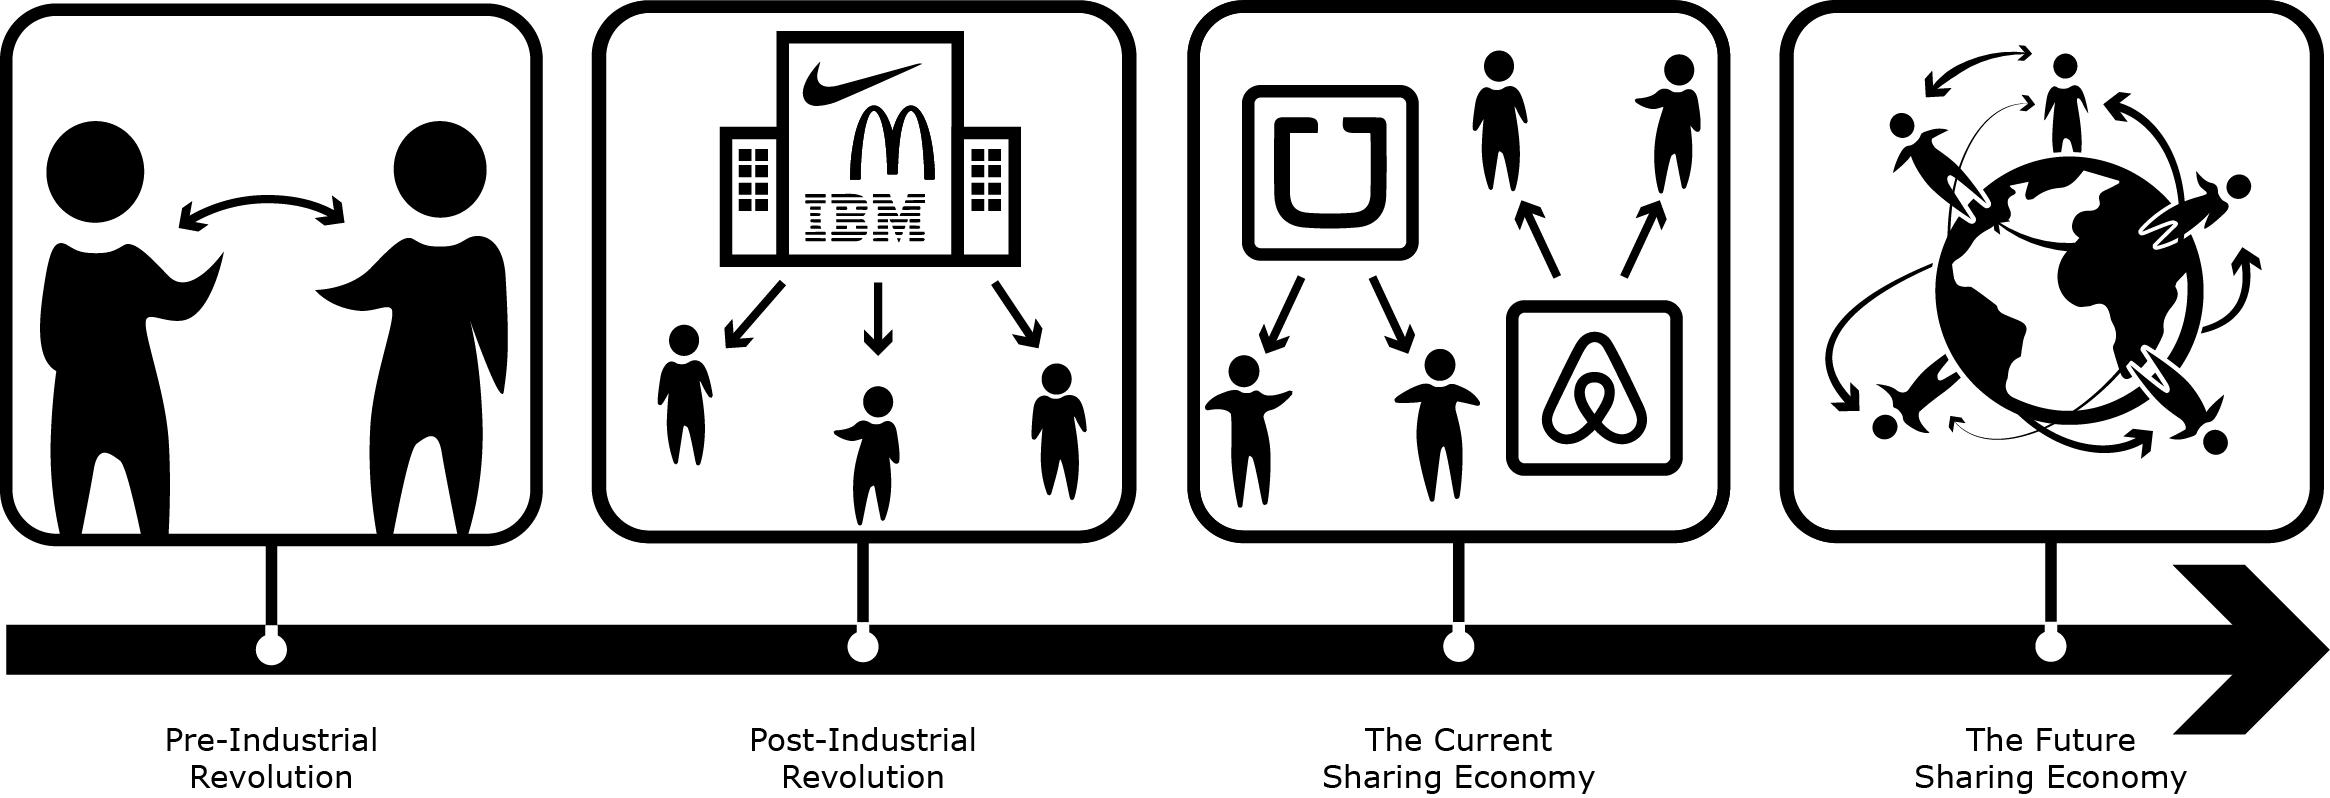
\includegraphics[width=0.8\textwidth]{images/economy.png}
    \caption{Evolution of the economy}
    \label{fig:economy}
\end{figure}

We envision a future in which collaborative consumption is possible without any intermediator. This
future requires a reputation system which is application agnostic, owned by noone and ruled by 
everyone. A distributed reputation system as a layer directly
on top of the internet. However this poses some challenges from a technical
point of view. Distributed system are intrinsically hard to control and regulate, which is both 
blessing and curse. No party can impose unfair rules on other users but it is also hard to prevent 
malicious users from sending wrong information across the network. \cite{HENDRIKX2015184} reviews
state-of-the-art reputation systems and finds that all commercial reputation systems are centralized.
Some of the scientific reputation systems are decentralized like EigenTrust 
\cite{kamvar2003eigentrust}, P-Grid \cite{aberer2003p} and RateWeb \cite{malik2009rateweb}, yet
they have not been proven to work in settings where high throughput, global scaling are required 
which is the case for a global reputation system. Distributed, secure and globally scalable systems
remain an unsolved problem.

% 5. This master thesis was written in the context of the blockchain lab at TU Delft which has a long history of research on the topic of distributed reputation systems. The research is targeted at Tribler, a secure BitTorrent client which is aimed at protecting against free-riders.
% BarterCast

This report is related to research done at the Blockchain Lab at TU Delft, whose ambition it is to 
be the first to create a working solution for this problem. In many years of research multiple 
milestones have been reached. In \cite{meulpolder2009bartercast} we have solved the free-riding 
problem in the peer-to-peer file-sharing context with a reputation system that tracks uploads and 
downloads. With TrustChain \cite{OTTE2017} we have created our own blockchain fabric for bandwidth
as a currency which builds on the previous work and adds tamper-proof recording and immutable history
to the reputation system. All work is implemented in Tribler, a BitTorrent client with Tor-like 
layered anonymity. The implementation allows for testing of research ideas with real users in 
production environments. 

This work specifically will be concerned with the agreement on reputation in the network and closely
related to that the dissemination of records of interactions. We
will enlarge on the problem description in the next chapter. Afterwards the problem will be defined
formally and analyzed in the bounds of the definition. Before proposing a solution, some existing
approaches for recording and dissemination of data will be discussed in chapter. Next, we define a
solution based on the TU Delft blockchain fabric TrustChain and propose a specific mechanism of 
using such a fabric. Finally, we prove the correctness and scalability properties of the fabric in
experimental analysis, before concluding and making suggestions for further research.